\documentclass{beamer}
\usepackage[MeX]{polski}
\usepackage[utf8]{inputenc}
\usepackage{graphicx}

%opening
\title{Bylica roczna}
\author{Michał Kozłowski}
\date{\today}
\institute{UWM}

\begin{document}

\frame{\titlepage}
	
\begin{frame}{Wstęp}
	\begin{center}
	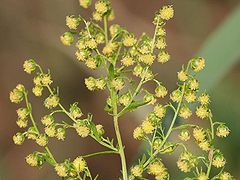
\includegraphics[scale = 0.6]{grafika/ilustracja.jpeg}
	%\frametitle
	\end{center}
	Bylica roczna (\textit{Artemisia annua} L.), lub też \textit{Artemisia chamomilla}\cite{site2} – gatunek roślin z~rodziny astrowatych (\textit{Compositae}~Gis.).
\end{frame}

\begin{frame}{Systematyka}
	\centering
	\begin{table}
		\begin{tabular}{lc}
		Domena&eukarionty\\ \pause
		Królestwo&rośliny\\ \pause
		Klad&rośliny naczyniowe\\ \pause
		Klad&Euphyllophyta\\ \pause
		Klad&rośliny nasienne\\ \pause
		Klasa&okrytonasienne\\ \pause
		Klad&astrowe\\ \pause
		Rząd&astrowce\\ \pause
		Rodzina&astrowate\\ \pause
		Podrodzina&Asteroideae\\ \pause
		Rodzaj&bylica\\ \pause
		Gatunek&bylica roczna\\
		\end{tabular}
	\end{table}
	\textit{ (dane ze strony \cite{site1}) }
\end{frame}

\begin{frame}
	\frametitle{Występowanie}
	
	Według encyklopedii roślin \cite{site3}, bylica roczna występuje:
	
	\begin{itemize}
		\item w środkowej i południowej Europie
		\pause
		\item Turcji \pause
		\item południowej Rosji \pause 
		\item Palestynie \pause 
		\item Syrii \pause
		\item Iranie \pause
		\item Afganistanie \pause
		\item Pakistanie \pause
		\item Indiach \pause
		\item południowych Chinach
	\end{itemize}
\end{frame}

\begin{frame}
	\frametitle{Występowanie}
	\begin{itemize}
		\item Została introdukowana w~Kanadzie i~Stanach Zjednoczonych. \pause
		\item W Polsce rośnie także jako zadomowiony antropofit.\cite{ksiazka}
	\end{itemize}
\end{frame}

\begin{frame}
	\frametitle{Morfologia}
	\begin{itemize}
		\item
		\textbf{Pokrój}
		Roślina jednoroczna dorastająca do 30–200 (wyjątkowo do 300) cm wysokości.
		\pause
		\item
		\textbf{Łodyga}
		Zazwyczaj jedna łodyga, wyprostowana, zielona, z~wiekiem zmieniająca barwę na~czerwonobrązową, naga lub~słabo owłosiona.
		\pause
		\item
		\textbf{Liście}
		Naprzemianległe. Mają jasnozieloną barwę. Mają 2–5 (wyjątkowo do 10) cm długości oraz 2–4~cm szerokości.
		\end{itemize}
\end{frame}

\begin{frame}
	\frametitle{Morfologia}
	\begin{itemize}
		\item
		\textbf{Kwiaty}
		Drobne, zwisające koszyczki kwiatowe, na~licznych odgałęzieniach zebrane w~groniasty kwiatostan. \pause
		\item
		Każdy koszyczek kwiatowy ma~średnicę około~2~mm. U~podstawy każdego koszyczka znajduje się 6 ciemnozielonych podsadek.
		\pause
		\item
		\textbf{Owoce}
		Niełupki.
	\end{itemize}
	\centering
	\textit{ (dane ze strony \cite{site3}) }
\end{frame}

\begin{frame}
	\frametitle{Gatunki podobne}
	Od Artemisia biennis Willd. różni się:
	\begin{itemize}
	\item podwójnie lub potrójnie pierzastymi liśćmi 
	\pause
	\item bardziej rozpierzchłymi kwiatostanami
	\end{itemize}
\end{frame}

\begin{frame}
	\frametitle{Biologia i ekologia}
	\begin{itemize}
		\item Roślina wiatropylna
		\pause
		\item Kwitnie od późnego lata do~jesieni.
		\pause
		\item Kwiaty są bezwonne, chociaż liście wydzielają słodki aromat
	\end{itemize}
\end{frame}

\begin{frame}
	\frametitle{Zastosowanie}
Zawiera substancje, które są~pomocne w~leczeniu malarii.
\end{frame}

\begin{frame}
	\frametitle{Bibliografia}
	\begin{thebibliography}{9}
		\bibitem{site1}
		P.F.Stevens: Angiosperm Phylogeny Website 2001 http://www.mobot.org/MOBOT/research/APweb/
		\bibitem{site2}
		Artemisia annua L. The Plant List (2014) http://www.theplantlist.org/tpl1.1/record/gcc-39740
		\bibitem{site3}
		Artemisia annua – Detail. Encyclopedia of~Life. (2014) http://eol.org/pages/469710/details
		\bibitem{ksiazka}
		Z. Mirek, H. Piękoś-Mirkowa, A. Zając, M. Zając: \textit{Krytyczna lista roślin naczyniowych Polski.} Instytut Botaniki PAN im. Władysława Szafera w~Krakowie, 2002
		
	\end{thebibliography}
\end{frame}


\begin{frame}
	\frametitle{Koniec}
	\begin{center}
	Dziękuję za uwagę!
	\end{center}
\end{frame}	
	
\end{document}
